\documentclass{jarticle}
\usepackage{robomech}
\usepackage[dvipdfmx]{graphicx}
\usepackage{here}
\usepackage{url}
\usepackage{comment}
% \usepackage{multirow}

\begin{document}
\makeatletter
\title{視覚と行動の end-to-end 学習により経路追従行動を\\オンラインで模倣する手法の提案}
{―実環境における経路選択機能の検証と学習時間の短縮化の検討―}
{A proposal for an online imitation method of path-tracking
behavior by end-to-end\\ learning of vision and action}
{-Verification of route selection function in a real environment and study of reducing learning time-}

\author{
% \centering
\begin{tabular}{lll}
 \centering
 \hspace{1zw}○学\hspace{0.7zw} 藤原柾(千葉工大)&\hspace{0.5zw}学\hspace{1zw}春山健太(千葉工大)
 \hspace{2zw}馬場琉生(千葉工大)\\
%  \hspace{4zw}馬場琉生(千葉工大)&\hspace{4zw} \hspace{1.2zw} 高橋佑樹(千葉工大)\\
%  \hspace{2zw}正\hspace{2zw}橋佑樹(千葉工大)& \hspace{1zw}春山健太(千葉工大)\\
 \hspace{2zw}正\hspace{1zw}上田隆一(千葉工大)& \hspace{0.5zw}正\hspace{1zw}林原靖男(千葉工大)&\\
 % ※協賛・後援団体の会員資格で発表される場合は「正・学」は不要です。
 \end{tabular}
 % &\\
 \vspace{1zh} \\
 \begin{tabular}{l}
{\small Masaki FUJIWARA, Chiba Institute of Technology, s19c1101ga@s.chibakoudai.jp}\\
{\small Kenta HARUYAMA, Ryusei BABA,}\\
% {\small Kenta HARUYAMA, Ryusei BABA, Yuki TAKAHASHI,}\\
{\small Ryuichi UEDA and Yasuo HAYASHIBARA, Chiba Institute of Technology}\\
%  {\small [Authors' names and Affiliations: Times New Roman, 9pt]}
\end{tabular}
}
\makeatother

\abstract{ \small 
We have proposed an online imitation method of path-following behavior by end-to-end learning of visual actions. However, the proposed method aims at orbiting a fixed path and cannot dynamically change the path in order to move the robot to the destination. Therefore, in this study, we add a route selection function so that the robot can move to any destination. We attempt to solve the problem of long learning time, which was identified through preliminary experiments in a real environment, by trying two approaches. In addition, we will verify the effectiveness of the route selection function through experiments in a real environment.
}

\date{} % 日付を出力しない
\keywords{Autonomous mobile robot, Navigation, End-to-end learning}

\maketitle
\thispagestyle{empty}
\pagestyle{empty}

\small
\section{緒言}%===========================
我々は, 入力データから出力を直接生成するend-to-end学習により, 経路追従行動をロボットの視覚に当たるカメラ画像に基づいてオンラインで模倣する手法を提案し, 有効性を実験により検証してきた\cite{okada1}\cite{okada2}(以下, 「従来手法」と称する). 加えて, この岡田らの従来手法に経路を選択する機能の追加を提案し, シミュレータ上での実験により, 有効性を検証してきた\cite{mech}. 
% 本稿では, 経路選択機能に関する実験をシミュレータ上から実環境に移す際に, 問題となった学習時間の長さについて, 2つのアプローチにより解決を図る. さらに, 実環境において経路選択機能の有効性を検証することを目的とする.
従来手法は, 測域センサやオドメトリなどを入力とする地図を用いたルールベース制御器による走行を模倣学習し, 似た行動を画像を用いて行う手法である. なお, 地図を用いたルールベース制御器は, ROS Navigation\_stack\cite{nav}へ目標位置(waypoint)の指示を行うwaypoint\_nav\cite{waypoint}を組み合わせたものである. この手法は, 多くの研究\cite{bojarski}\cite{moridian}\cite{hawke}が人間のドライバーが操作するステアリング角度を用いて模倣学習を行っていたのに対して, オンラインで自動的にデータセットを収集して模倣学習を行う点で異なっているといえる.

この手法は, 学習を行った一定の経路を走行できるが, 目的地に対して経路を動的に選択して走行することはできない. それをするためには, ネットワークの入力に新たな要素の追加が必要となる. 
新たな要素として, カメラ画像とステアリング角度に条件を加えて学習を行う条件付き模倣学習の研究が現在までにいくつか行われている. Felipeら\cite{felipe}やHawkeら\cite{hawke}は, 前方カメラ画像に加えて方向を指示するコマンドを入力とするネットワークを用いて模倣学習を行った. そのため, 前報\cite{mech}ではネットワークへ条件を追加し, 分岐路において任意の経路を選択する機能の追加を提案した. また, 実験により有効性を検証した. しかし, 有効性の検証はシミュレータ上のみでしか確認しておらず, 実環境においては未確認であった. 

そこで本稿では, 前報\cite{mech}で追加した経路選択機能の有効性を実環境において検証する. さらに, 実験で問題となった学習時間の長さについて, 2つのアプローチにより学習時間を短縮することを目的とする.

条件付き模倣学習により, 学習済みモデルによる走行時において経路を制御できるようになると, 自律走行を行う手段が地図を用いたルールベース制御器と模倣学習など, 複数持つことができる. たとえば, 自律走行の手段を切り替えることでロバスト性の向上が期待できる.
% また, 実環境における実験のための学習時間の短縮化の検討を行う.
% \par
% カメラ画像とステアリング角度に, 条件を加えて学習を行う条件付き模倣学習の研究は, 現在までにいくつか行われている. Felipeら\cite{felipe}は前方カメラ画像, ステアリング角度, 角速度と「continue」, 「left」, 「straight」, 「right」からなるコマンドを入力としたネットワークを用いて模倣学習を行った. そして, 実環境と都市環境のシミュレータ上で, 模倣学習のテスト時においてもコマンドによって制御可能であることを確認している. また, Hawkeら\cite{hawke}は3つの前方カメラ画像と「go straight」, 「turn left」, 「turn right」からなるコマンドを入力とする構造のモデルを用いて, 実環境での複雑な都市環境というシナリオで, 意思決定が可能なモデルをわずか30時間の学習データで学習可能であることを示している.
% \par
% そこで本稿では, 従来から提案する経路追従行動を模倣する手法に対して, 条件を加えることで経路を選択する機能の追加を試みる. これにより, 模倣学習のテスト時においても, \reffig{fig: fig1}のような分岐路で, 
% 「直進」, 「左折」などのコマンドによる制御で任意の経路への移動を可能にすることを目指す.

% \vspace{3mm}

% \begin{figure}[H]
%  \centering
%   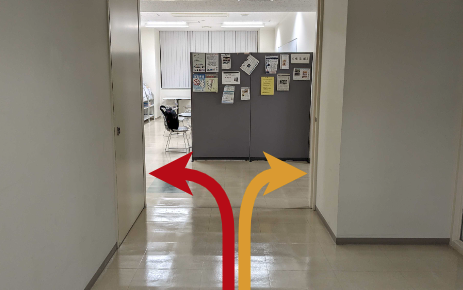
\includegraphics[height=30mm]{road.png}
%   \vspace*{-4mm}
%   \caption{A fork in the road where the direction of moving is not unique}
%   \label{fig: fig1}
% \end{figure}

% \vspace{-4mm}

\section{従来手法}
岡田らの従来手法に関して紹介する. \reffig{fig: fig2}に経路追従行動を視覚に基づいてオンラインで模倣するシステムを示す. 手法は機械学習により, 学習器の訓練を行う「学習フェーズ」と訓練した結果を検証する「テストフェーズ」に分かれる.

\subsection{学習フェーズ}
学習フェーズは, 模倣学習によって学習器の訓練を行うフェーズである. 測域センサとオドメトリを入力とする地図を用いたルールベース制御器で自律走行する. この経路追従行動を, カメラ画像を用いたend-to-endで模倣学習する. 前報\cite{okada2}で述べたように, 岡田らの手法ではデータセットの収集方法にいくつかの種類がある. 本稿では, その中で最も経路追従の成功率が高い手法を用いてロボットに模倣学習をさせる.

\subsection{テストフェーズ}
テストフェーズは, 訓練後の学習結果を評価するフェーズである. 学習器にカメラ画像を入力し, 出力されるヨー方向の角速度を用いて自律走行する.

\begin{figure}[H]
  \centering
   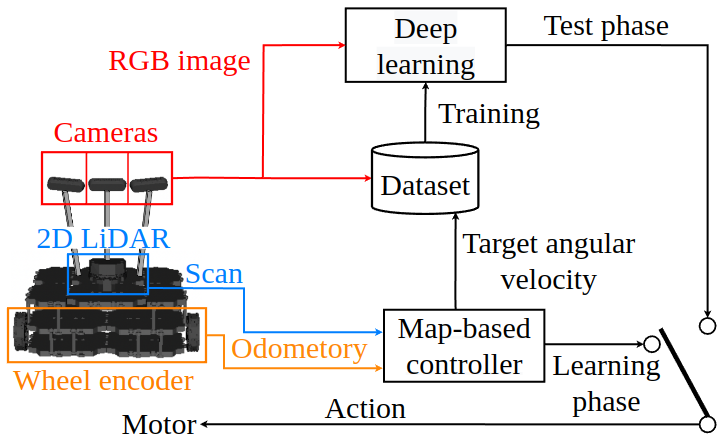
\includegraphics[width=85mm]{system.png}
   \vspace*{-4mm}
   \caption{Imitation learning system of learning phase}
   \label{fig: fig2}
 \end{figure}

\section{経路選択機能の追加}
経路選択機能の追加を目的として, データセットと学習器の入力へ, 目標とする進行方向(以下, 「目標方向」と称する)を追加する. なお, 追加した要素以外は従来手法と同様である. \reffig{fig: fig3}に提案手法のシステムを示す. 学習フェーズでは, 地図を用いたルールベース制御器で自律走行しながら, 角速度, カメラ画像に新たに目標方向をデータセットに加える. テストフェーズでは, 学習器にカメラ画像に加えて目標方向を外部から入力する. 本稿では議論しないが, 最終的に目的地までカメラ画像のみで自律走行させることを目標としているため, 目標方向を自動的に作成する仕組みが必要となる. これに関しては, カメラ画像からトポロジカルマップのどのノード上に到達したかを判定し, 目標方向を自動的に切り替えるパッケージを作成している\cite{graph}.

\begin{figure}[H]
  \centering
   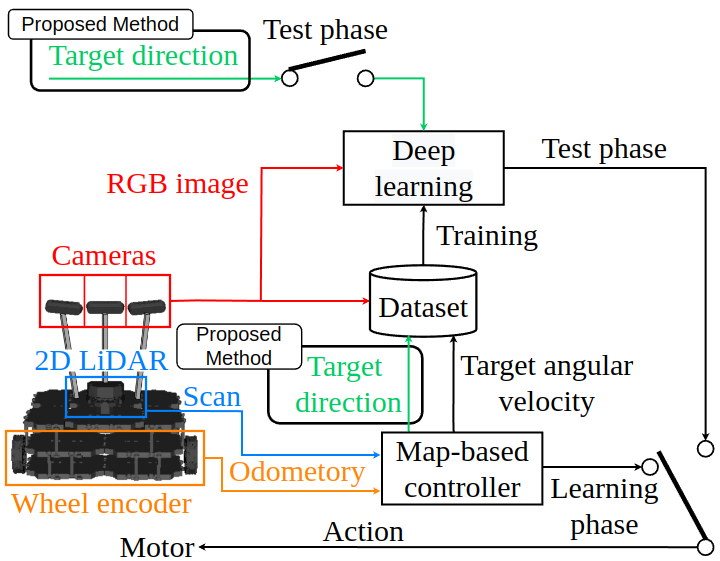
\includegraphics[width=85mm]{system2.png}
   \vspace*{-4mm}
   \caption{Imitation learning system of test phase}
   \label{fig: fig3}
 \end{figure}

\section{ネットワークとデータ形式}
\reffig{fig: fig4}に経路選択機能を追加したネットワーク, \reftab{tbl: table1}にハイパーパラメータを示す. 
先行研究に倣って, 前報で用いたネットワークの出力部へ2つの層を追加した. この層に目標方向として, \reftab{tbl: table2}
% のワンホットベクトルで
に表されるデータを入力する. なお, 前報\cite{mech}では「Continue」, 「Go straight」, 「Turn left」, 「Turn right」からなる4つのコマンドを用いていたが, 「Continue」と「Go straight」のコマンドに対応する行動がほぼ同一であったため, 本稿ではコマンドを1つ減らし, 3コマンドとしている. 
% \reffig{fig: fig5}はそれぞれの進行方向を示している.

\begin{figure}[h]
  \centering
   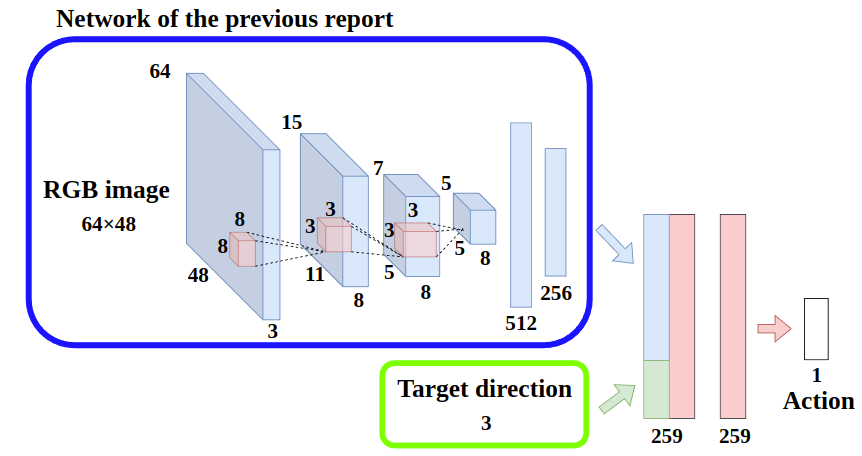
\includegraphics[width=85mm]{network.png}
   \vspace*{-4mm}
   \caption{Structure of network}
   \label{fig: fig4}
 \end{figure}

 \begin{table}[h]
  \caption{Parameters of network}
  \label{tbl: table1}
  \centering
  \footnotesize
  \vspace{2mm}
  \begin{tabular}{|c|c|}
   \hline
   Input data & 
   \begin{tabular}{c}
    Image (64×48 pixels, RGB channels), \\ Target direction
   \end{tabular}
   \\\hline
   Optimizer & 
   \begin{tabular}{c}
   Adam(alpha = 0.001, beta1 = 0.9, \\beta2 = 0.999, eps = 1$e^{-2}$) 
  \end{tabular}
  \\\hline 
  Loss function & Softmax-cross-entropy\\\hline
  Output data & Angular velocity\\
   \hline
  \end{tabular}
\end{table}

\begin{table}[H]
 \caption{Target direction and data for imitation learning}
 \label{tbl: table2}
 \centering
 \footnotesize
 \vspace{2mm}
 \begin{tabular}{|c|c|}
  \hline
	Target direction & Data \\\hline
  Go straight & [100, 0, 0] \\\hline
  Turn left & [0, 100, 0] \\\hline
  Turn right & [0, 0, 100] \\
  \hline
 \end{tabular}
\end{table}

% \begin{figure}[h]
%   \centering
%   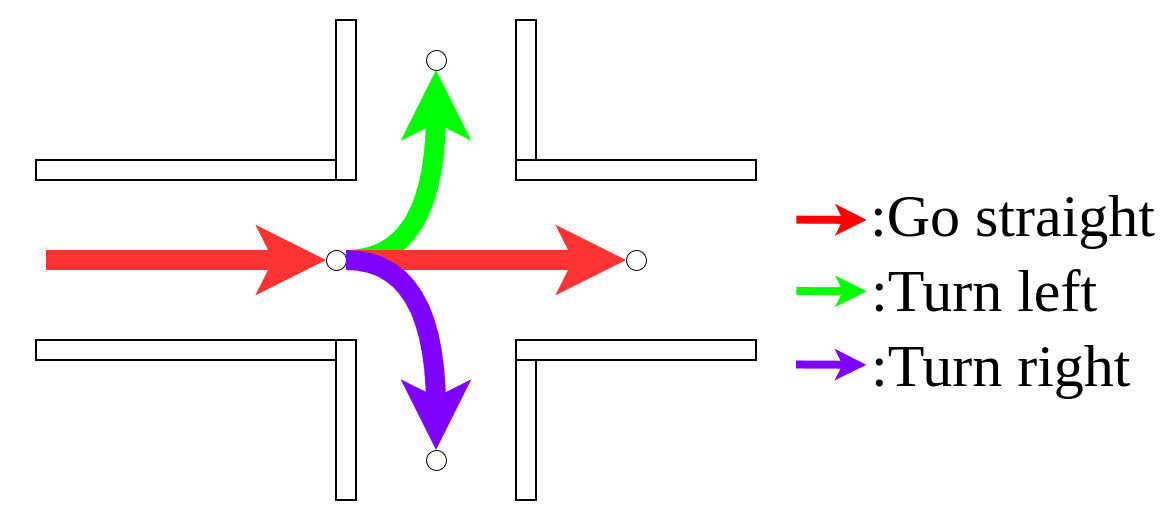
\includegraphics[width=75mm]{direction.png}
%   \vspace*{-4mm}
%   \caption{Target direction}
%   \label{fig: fig5}
% \end{figure}

% \newpage
\section{提案手法の検証実験}
前報\cite{mech}で行った実験2を実環境に移して行う.
% 構築したシステムで, 目標方向に従って経路を選択できることを実環境の実験により確認する. 
\subsection{実験装置}
% \subsubsection{コンピュータ}
ロボットは, \reffig{fig: fig6}に示すような3つのカメラを搭載したロボットを用いる. また, 実験は千葉工業大学津田沼キャンパス2号館3階で行った.

\begin{figure}[h]
  \centering
   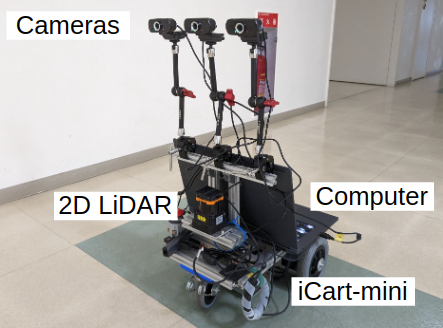
\includegraphics[width=50mm]{gamma3.png}
   \vspace*{-4mm}
   \caption{Experimental setup}
   \label{fig: fig6}
 \end{figure}

 \subsection{実験方法}
 \reffig{fig: fig7}に示すようなA,Bの三叉路で全ての侵入方向と抜け出す経路を含めるように, 前報\cite{mech}の実験2と同様の経路を繰り返し走行させる. 学習を60000step実行後, テストフェーズに移行する. テストフェーズでは, 学習フェーズと同様の経路を, 目標方向による制御によって正しく走行できるか評価する. しかし, 実験を行ったのは1回のみである. 実験が1回のみなのは, 学習時間の長さが問題になったためである. 具体的には, 実験におよそ7時間を要し, バッテリなどの関係で1日に1, 2時間が限界であったため, 1回の実験に1週間かけて行う必要があった.

 \begin{figure}[h]
  \centering
   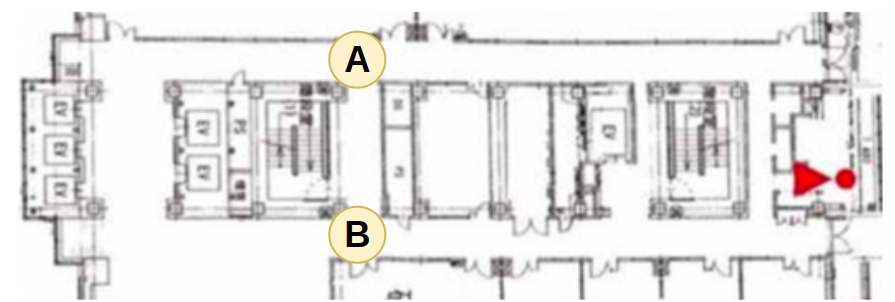
\includegraphics[width=70mm]{tsudanuma2.png}
   \vspace*{-4mm}
   \caption{Experimental environment}
   \label{fig: fig7}
 \end{figure}

\subsection{実験結果}
実験結果を\reffig{fig: fig8}に示す. この図は, それぞれの侵入方向に対して正しい経路を選択し, 走行できた回数を表している. 目標方向に従って9/12回(75\%), 正しい経路を選択する様子が見られた.

\begin{figure}[h]
  \centering
   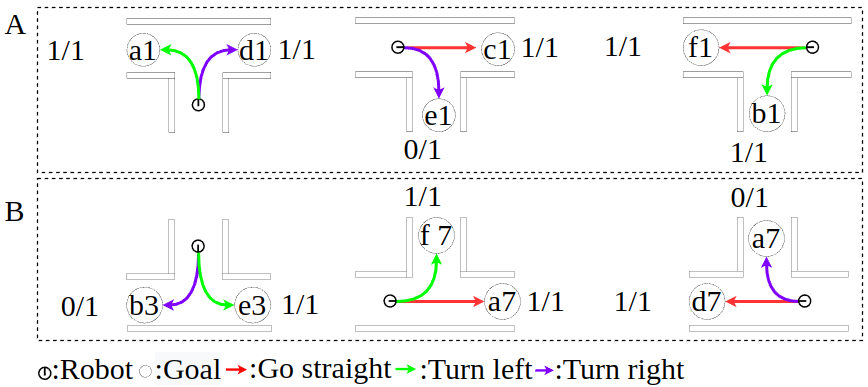
\includegraphics[width=80mm]{60000step_real2.png}
   \vspace*{-4mm}
   \caption{Number of times a correct path was selected}
   \label{fig: fig8}
 \end{figure}

\section{学習時間の短縮化の提案}
\subsection{問題}
% 前章で述べたように, シミュレータ上での実験により提案手法が有効だと
前報\cite{mech}で行った実験により, シミュレータ上では提案手法が有効だと確認している. そのため, 5章で述べたように, 実環境における提案手法の有効性を検証することを試みた. しかし, 学習時間の長さが問題となり, 評価を複数回行うことが困難であった. そのため, 学習時間の短縮化に関して2つのアプローチを提案し, 学習時間の削減の効果を実験により確認する.

\subsection{学習ステップ数の削減による影響}
前報\cite{mech}のシミュレータ上で行った実験2と同様の条件で, 60000stepから10000stepに学習ステップ数を変更し, 実験を行った.
% \par 
実験結果を\reffig{fig: fig9}に示す. \reftab{tbl: table3}に侵入方向ごとの成功回数を合計した結果を示す.
表に示すように, 87/120回 正しい経路を選択する様子が見られた.
\par
60000stepの実験と成功率を比較すると約22\%ほどの差がある. これまで述べた提案手法では, 学習ステップ数を減らすことにより, 成功率が大幅に低下することが判明した. そのため, 後述する2つのアプローチを試みることで成功率の改善を図る.

\begin{figure}[h]
  \centering
   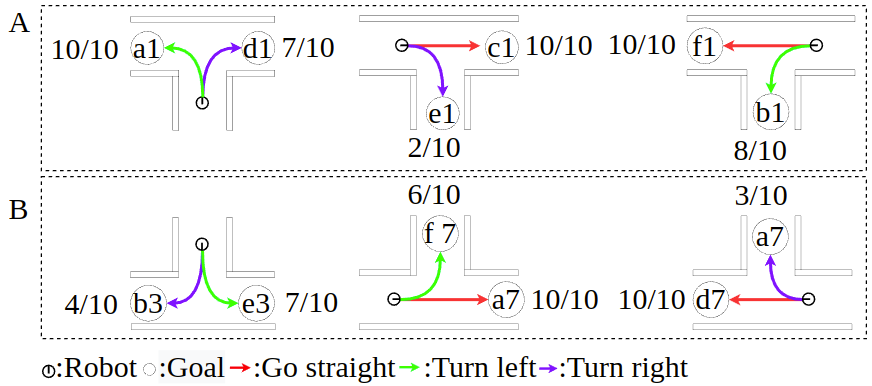
\includegraphics[width=85mm]{10000step.png}
   \vspace*{-4mm}
   \caption{Number of times a correct path was selected}
   \label{fig: fig9}
 \end{figure}

 \vspace{-8mm}

 \begin{table}[H]
  \caption{Experimental results}
  \label{tbl: table3}
  \centering
  \footnotesize
  \vspace{2mm}
  \begin{tabular}{|c|c|c|}
   \hline
   Experiment & Step & Total results \\\hline
   Exp.2 from \cite{mech} & 60000 & 113/120(94.2\%) \\ \cline{2-3}
  & 10000 & 87/120(72.5\%)\\
   \hline
  \end{tabular}
 \end{table}

\subsection{アプローチ1:データセットに加えるデータの割合の変更}
6.2章の実験における10000stepあたりのコマンドのデータ数を\reffig{fig: fig10}に示す. \reffig{fig: fig10}(a)より, 直進コマンドのデータ数が圧倒的に多く, 不均衡データであることが分かる.
不均衡データを調査したHaiboら\cite{haibo}によると, ほとんどの標準的な学習アルゴリズムがデータの不均衡により, パフォーマンスが大幅に低下すると述べている. そのため, オーバーサンプリングを行い, データの偏りを改善する. \reffig{fig: fig10}(b)に示すように, 左折と右折コマンドのデータを7倍に複製し, データセットへ加える. なお, データを何倍にするのが望ましいのか本稿では議論しない. 実験により, データセットに加えるデータ数の割合の変更が有効か検証する.

\begin{figure}[h]
  \centering
   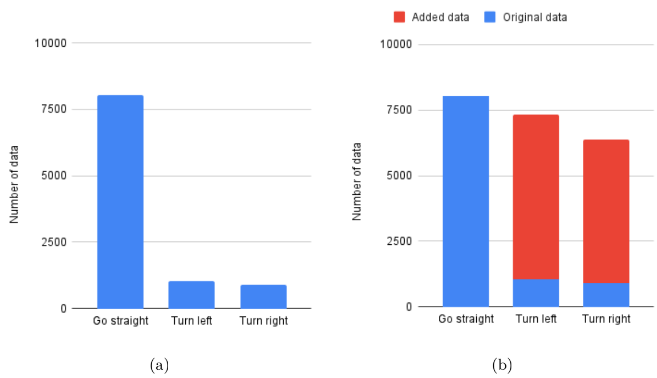
\includegraphics[width=87mm]{hist.png}
   \vspace*{-6mm}
   \caption{Number of data per command per 10000steps in conventional experiments}
   \label{fig: fig10}
 \end{figure}

\subsubsection{実験装置}
前報\cite{mech}で行った実験2のシミュレータ環境とロボットで実験を行った.

\subsubsection{実験方法}
前報\cite{mech}の実験2と同様の経路を繰り返し走行させる. 学習を10000step実行後, テストフェーズに移行し, 評価する. この一連の流れを10回行う.

\subsubsection{実験結果}
実験結果を\reffig{fig: fig11}に示す. \reftab{tbl: table4}に侵入方向ごとの成功回数を合計した結果を示す. 表に示すように, 99/120回 正しい経路を選択する様子が見られた. 6.2章の学習ステップ数を減らした結果と比べると成功率は高いが, 60000stepの実験と成功率を比較すると約12\%ほど差があり, アプローチ1を試みた結果では成功率が高いとは言い難いため, 次にアプローチ2を試みる.

\begin{figure}[h]
  \centering
   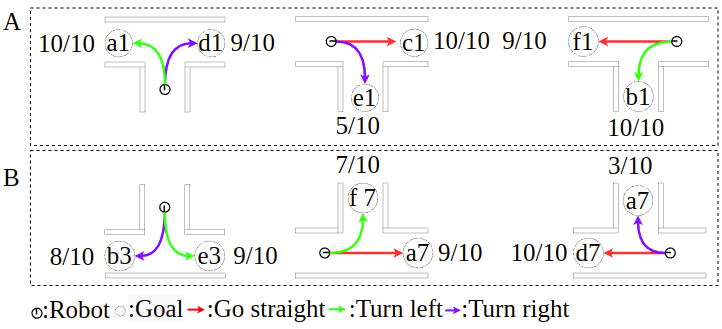
\includegraphics[width=85mm]{10000step_act1.0.png}
   \vspace*{-4mm}
   \caption{Number of times a correct path was selected}
   \label{fig: fig11}
 \end{figure}

 \vspace{-8mm}

 \begin{table}[H]
  \caption{Experimental results}
  \label{tbl: table4}
  \centering
  \footnotesize
  \vspace{2mm}
  \begin{tabular}{|c|c|c|}
   \hline
   Experiment & Step & Total results \\\hline
   Exp.2 from \cite{mech} & 60000 & 113/120(94.2\%) \\ \cline{2-3}
  & 10000 & 87/120(72.5\%)\\\hline
  Data 7 times & 10000 & 99/120(82.5\%)\\
   \hline
  \end{tabular}
 \end{table}

\subsection{アプローチ2:学習フェーズにおける積極的な蛇行}
清岡ら\cite{kiyooka}により, 目標経路上に加えて離れた状態を学習することが, テストフェーズでの走行において目標経路に復帰できるかに大きな影響を与えるため, 重要だとされている. そのため, より積極的に蛇行を行い, 目標経路から離れた状態を増加させることを検討する.
\par
訓練中の学習器へ画像を入力し, \reffig{fig: fig12}のように出力される角速度を1.5倍にする. その結果, 蛇行する頻度が高くなり, 目標経路から離れた状態をより多く学習できる可能性がある. なお, 得られた角速度を何倍にするのが望ましいのか本論文では議論しない. 実験により, 学習フェーズにおける積極的な蛇行が有効か検証する.

\begin{figure}[h]
  \centering
   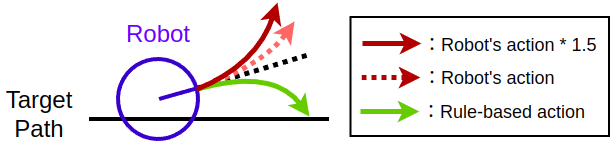
\includegraphics[width=85mm]{3action3.png}
   \vspace*{-4mm}
   \caption{Robot behavior}
   \label{fig: fig12}
 \end{figure}

\subsubsection{実験装置}
前報\cite{mech}で行った実験2のシミュレータ環境とロボットで実験を行った.

\subsubsection{実験方法}
6.3章と同様の条件で実験を行った.

\subsubsection{実験結果}
実験結果を\reffig{fig: fig13}に示す. \reftab{tbl: table5}に侵入方向ごとの成功回数を合計した結果を示す.
表に示すように, 109/120回 正しい経路を選択する様子が見られた. 

\begin{figure}[h]
  \centering
   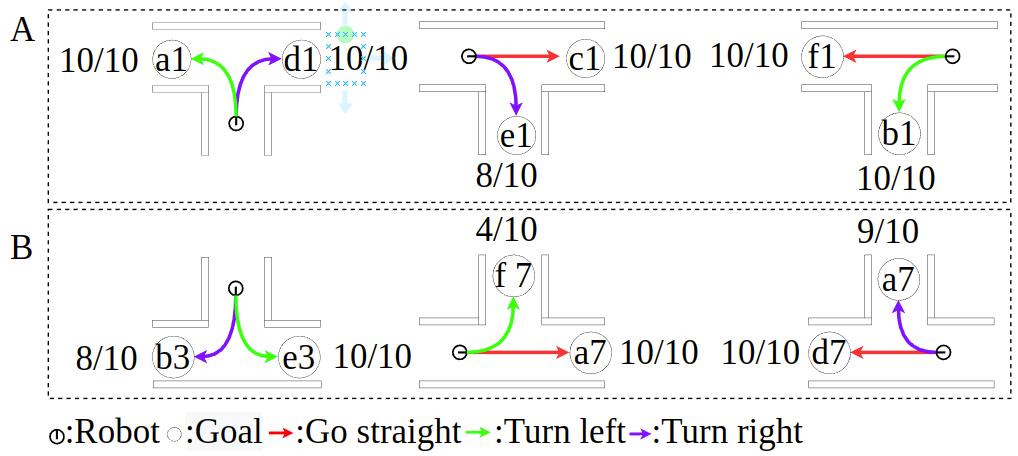
\includegraphics[width=85mm]{10000step_act1.5_2.png}
   \vspace*{-4mm}
   \caption{Number of times a correct path was selected}
   \label{fig: fig13}
 \end{figure}

 \vspace{-8mm}

 \begin{table}[H]
  \caption{Experimental results}
  \label{tbl: table5}
  \centering
  \footnotesize
  \vspace{2mm}
  \begin{tabular}{|c|c|c|}
   \hline
   Experiment & Step & Total results \\\hline
   Exp.2 from \cite{mech} & 60000 & 113/120(94.2\%) \\ \cline{2-3}
  & 10000 & 87/120(72.5\%)\\\hline
  Data 7 times & 10000 & 99/120(82.5\%)\\\hline
  Aggressive meandering & 10000 & 109/120(90.8\%) \\ \cline{2-3}
  & 20000 & 114/120(95\%)\\
   \hline
  \end{tabular}
 \end{table}

 6.3章のデータの割合の変更した結果と比べると成功率が改善していることが分かる. 以下に\reffig{fig: fig13}における成功率が低い場所と要因を示す.

 \begin{itemize}
  \item f7\\
  前報\cite{mech}で行った実験2と同様に, 予め設定した経路の最後であるため, データセットにf7のデータが加えられてから十分に学習がされていないおそれがある.
  \item a7, b3, e1\\
  これらは, 全て右折する場所である. \reffig{fig: fig10}より, 他のコマンドのデータと比較して右折コマンドのデータが少ないことが分かる. このことから, 右折コマンドのデータを十分に学習できていないおそれがある. 
 \end{itemize}
 
この2つの点から, 学習ステップ数を増やすと成功率が改善する可能性がある. そのため, 10000stepから20000stepに学習ステップ数を増やして実験した. 実験結果は, \reftab{tbl: table5}に示すように成功回数が 114/120回(95\%)となり, 成功率が60000stepの実験と同程度になった. このことから, 学習時間を短縮するための2つのアプローチにより, 学習のステップ数が約67\%削減できたといえる.

\subsection{実環境の実験}
5章で行った実験に2つのアプローチを追加して実験を行った. 実験装置は5章と同様である.

% \subsubsection{実験装置}
% 5.1章で示した環境とロボットで実験を行った.

\subsubsection{実験方法}
シミュレータ上で, まずは学習を10000step行い, その学習器を実環境でファインチューニングする. 学習フェーズでは, 前報\cite{mech}の実験2と同様の経路を繰り返し走行させる. 学習を10000step実行後, テストフェーズに移行し, 評価する. この一連の流れを10回行う.

\subsection{実験結果}
実験結果を\reffig{fig: fig14}に示す. 目標方向に従って 78/120回(65\%) 正しい経路を選択する様子が見られた. 前章までに行ってきたシミュレータ上での実験では, 成功率が90\%を超えていたが, 実環境での成功率は65\%と低かった. なお, 成功率が低い原因の解明には未だ至っていない. この問題の検討は, 今後の課題となっている.

\begin{figure}[h]
  \centering
   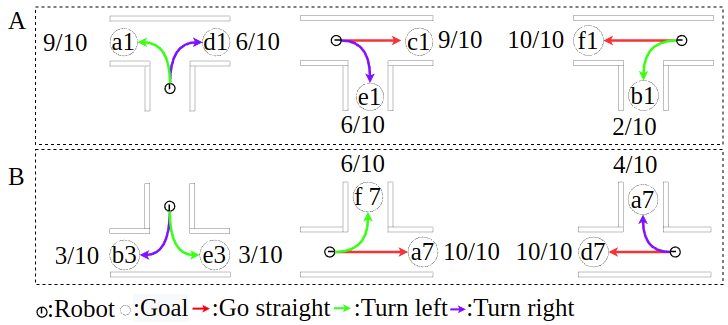
\includegraphics[width=85mm]{real_result.png}
   \vspace*{-4mm}
   \caption{Number of times a correct path was selected}
   \label{fig: fig14}
 \end{figure}

\section{結言}
本稿では, 経路追従行動をカメラ画像を用いた end-to-end 学習で模倣する岡田らの従来手法をベースに, データセットと学習器の入力へ目標方向を加えることで, 経路選択をする機能の追加を提案した. また, シミュレータ上での実験を実環境に移す際に, 問題となった学習時間の長さについて, 2 つのアプローチを試みることで学習時間を約67\%削減した. 加えて, 実環境での実験を行い, 有効性の検証を行った. 実験結果より, 学習器へ目標方向を与えることで, 指定した経路へ走行する挙動が確認できた.

% 本文:明朝体・9pt(欧文Times New Roman, 9pt)、文字間隔は1行26文字程度、行間隔は4.2mm程度にして下さ	い。

% \subsection{論文作成に関する注意事項を以下に示します。(中見出し:ゴシック体・9pt・強調文字・左寄せ)}%-----------
% \begin{itemize}
% 	\item 用紙サイズ:A4(210×297mm)とします。
% 	\item 用紙マージン:上下25mm。日本語表題から\textbf{\textit{Key Words}}までの1段組の部分は、左右25mm以上空けて下さい。本文からは2段組とし、左右15mm、段間は6mmとします。
% 	\item 文字のフォント、大きさ:\reftab{tbl: table1}を参照下さい。
% 	\item 図の画質:300dpi以上の画質の高いものにして下さい。
% 	\item 図・表のタイトル:図のタイトルには「Fig.\# English title」、表のタイトルには「Table \# English title」という形式を用い、文中ではそれぞれ「図\#」、「表\#」という表現にして下さい。
% 	\item グラフの軸タイトル:各軸のタイトルに変数記号だけを記述するのは避けて下さい。\reffig{fig: fig1}に示すように、軸を表す語句ならびに単位を記入して下さい。
% 	\item 式:以下に示すように、右寄せで番号をふり、式は中央に配置して下さい。文中では「\refeqn{eqn: eq1}」と表現して下さい。
	
% 	\begin{equation}
% 		M\ddot{r}_{str1} + F_{frk} = Mg
% 		\label{eqn: eq1}
% 	\end{equation}

% 	\item 単位:SI単位系とします。
% 	\item 本文中に文献を引用する場合、引用を表す語句や文の後ろに文献番号(例えば\cite{Shinjuku98})を振って下さい。文献を主語や目的語などに用いる場合、「文献\cite{Shinjuku98}では、・・」などのようにして、番号のみの表現を避けて下さい。
% 	\item 連名の場合には講演発表者氏名の前に○印をつけて下さい。
% 	\item 作成した論文はPDFファイル形式に変換し、PDFファイルのみを学会本部へ提出して下さい。PDFファイルの提出は本講演会ホームページ記載のアップロードのページの指示に従って下さい。
% 	\item[]
% 	\item[※] ただし、PDFファイルの容量は2MB以下、論文のページ数は2頁以上4頁以下とします。なお、印刷原稿の提出は不要ですので、郵送しないで下さい。
% 	\item[※] 講演番号、講演会名、ページ番号は記載しないようにして下さい。
% \end{itemize}

% %※ ただし、PDFファイルの容量は2MB以下、論文のページ数は2頁以上4頁以下とします。なお、印刷原稿の提出は不要ですので、郵送しないで下さい。

% %※ 講演番号、講演会名、ページ番号は記載しないようにして下さい。


% \begin{table}[h]
%  \caption{Type size and typefaces for papers}
%  \label{tbl: table1}
%  \centering
%  \footnotesize
%  \begin{tabular}{|p{7zw}|c|c|c|}
%   \hline
% 	適用場所	&日本語	&欧文 \\\hline
% 	標準のフォント	&明朝体 9pt	&Times New Roman 9pt \\\hline
% 	日本語表題	&ゴシック体 14pt	&Arial 14pt \\\hline
% 	日本語副表題	&ゴシック体 12pt	&Arial 12pt \\\hline
% 	英語表題	&-&Times New Roman 12pt \\\hline
% 	英語副表題	&-&Times New Roman 10pt \\\hline
% 	日本語著者名	&明朝体 10pt &-\\\hline
% 	英語著者名	&-&Times New Roman 9pt \\\hline
% 	アブストラクト・キーワード	&-&Times New Roman 9pt \\\hline
% 	大見出し	&ゴシック体 10pt	&Arial 10pt \\\hline
% 	中見出し	&ゴシック体 9pt	&Arial 9pt \\\hline
% 	図・表の番号・タイトル	 &-&Times New Roman 9pt \\\hline
% 	文献	&明朝体 8pt	&Times New Roman 8pt \\
%   \hline
%  \end{tabular}
% \end{table}

% \begin{figure}[h]
%  \centering
%   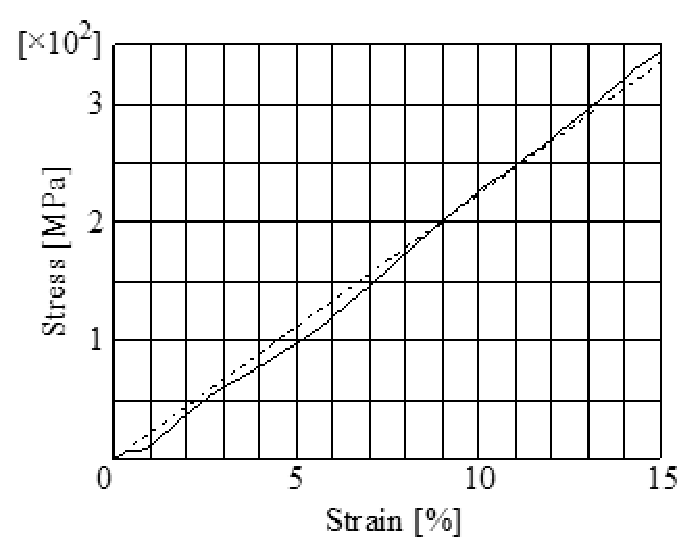
\includegraphics[height=38mm]{fig1.eps}
%   \vspace*{-4mm}
%   \caption{Tensile stress-strain diagram}
%   \label{fig: fig1}
% \end{figure}


\footnotesize
\begin{thebibliography}{99}

% \bibitem{Shinjuku98}
% 新宿大五朗,渋谷次郎,東京 学,``キャスティングマニピュレーションに関する研究(第1報,可変長の紐状柔軟リンクを有するマニピュレータの提案とそのスイング制御法)'',{\it 機論C編}, vol.64-626, pp.3854--3861, 1998.

% \bibitem{Shinjuku99}
% Shinjuku, D., Shibuya, J. and Tokyo, M., ``Swing Motion Control of Casting Manipulation,'' {\it IEEE Control Systems}, vol.19-4, pp.56--64, 1999.

\bibitem{okada1}
岡田眞也,清岡優祐, 上田隆一,林原靖男“視覚と行動の : end-to-end 学習により経路追従行動 をオンラインで模倣する手法の提案”,計測自動制御学会 SI 部門講演会 SICE-SI2020 予稿集,pp.1147–1152(2020)

\bibitem{okada2}
岡田眞也,清岡優祐,春山健太,上田隆一,林原靖男:“視覚と 行動の end-to-end 学習により経路追従行動 をオンラインで 模倣する手法の提案 -経路追従行動の修正のためにデータセッ トを動的に追加する手法の検討”,計測自動制御学会 SI 部門 講演会 SICE-SI2021 予稿集,pp.1066-1070(2021)

\bibitem{bojarski}
Bojarski, Mariusz,et al. “End to end learning for self- driving cars.”arXiv:1604.07316(2016)

\bibitem{moridian}
Moridian, Barzin, Anurag Kamal, and Nina Mahmoudian. "Learning navigation tasks from demonstration for semi- autonomous remote operation of mobile robots." 2018 IEEE International Symposium on Safety, Security, and Rescue Robotics (SSRR). IEEE, (2018)

\bibitem{felipe}
Felipe Codevilla et al.“end-to-end driving via conditional imitation learning.” arXiv: 1710.02410(2018)

\bibitem{mech}
春山健太, 藤原柾, 清岡優祐, 岡田眞也, 上田隆一, 林原靖男,“視覚と行動の end-to-end 学 習により経路追従行動をオンラインで模倣する手法の提案―経路選択機能の追加―“, 日 本機械学会ロボティクス・メカトロニクス講演会’22 予稿集,(2022).

\bibitem{hawke}
Jeffrey hawke et al. ”urban driving with conditional imitation learning”. arxiv: 1912.00177, 2019.

\bibitem{nav}
ros-planning, navigation レポジトリ. \\\url{https://github.com/ros-planning/navigation.}\\
(最終閲覧日:2月9日)

\bibitem{waypoint}
waypoint\_nav レポジトリ. \\\url{https://github.com/open-rdc/waypoint_nav.git.}\\
(最終閲覧日:2月9日)

\bibitem{graph}
weighted\_graph レポジトリ. \\\url{https://github.com/masakifujiwara1/weighted_graph.git}\\
(最終閲覧日:2月9日)

\bibitem{kiyooka}
清岡優祐, 岡田眞也, 岩井一輝, 上田隆一, 林原靖男, “視覚と行動の end-to-end 学習により経路追従行動をオンラインで模倣する手法の提案―
データセットと生成された経路追従行動の解析 ―”, 計測自動制御学会 SI 部門講演会 SICE-SI2021 予稿集, pp.1071–1075(2021)

\bibitem{haibo}
He, Haibo, and Edwardo A. Garcia. ”Learning from imbalanced data.” IEEE Transactions on knowledge and data engineering 21.9 (2009): 1263-1284.

\end{thebibliography}

\normalsize
\end{document}
